\chapter{Desenvolupament d’un entorn IoMT simulat}
Per al desplegament d’un entorn IoMT simulat seguint l’arquitectura explicada a \ref{sec:Topologia} he elaborat un entorn a través de contenidors Docker i l’orquestrador per defecte Docker Compose.

Per a la realització dels clients, que representen el trànsit benigne, he utilitzat una imatge d’Ubuntu, aquesta ha estat modificada (i renombrada com a mqttclient) on mitjançant el gestor de paquets APT  s'ha instal·lat mosquitto-clients 2.0.20 {ref imatge}. Amb aquesta aplicació podem fer actuar aquest contenidor d'Ubuntu com un client MQTT i tenir les seves funcions principals com subscriure’s i publicar a un tòpic d’un broker concret i utilitzar totes les funcionalitats descrites. {ref mosquitto}

També he instal·lat Python 3.13.2 i Paho-mqtt 2.0.0 \cite{pahoexp} per a poder generar paquets de forma personalitzada. Amb aquesta llibreria de Python podem modificar aspectes molt més concrets de les nostres connexions MQTT i paquets, canviant els valors de les dades o la freqüència d’enviament de les publicacions. Gràcies a aquesta eina, al ser una llibreria de Python, podem córrer els clients de manera automatitzada utilitzant les eines pròpies del llenguatge.

També he instal·lat les eines net-tools i iputils per tal de poder monitoritzar l’estat dels contenidors i fer comprovacions de connectivitat.


Pel que fa al Broker, he utilitzat l’imatge oficial de mosquitto anomenada eclipse-mosquitto (versió 2.0.21) \cite{mosquittoimg}. Aquesta permet l’ús del contenidor com a broker MQTT en les seves versions 3.1 i 5.1.1 amb totes les funcionalitats de les quals disposa la versió local \ref{sec:mosquitto}.

Respecte a configuració de Docker, he mapejat els ports 1883 i 8883 perquè en establir una connexió TCP a un d’aquests ports de l'hipervisor et dirigeixi al mateix port d’aquest contenidor en concret. També he generat 3 volums compartits amb l'hipervisor:
\begin{itemize}
    \item \textbf{Config:} on s’ubica el fitxer de configuracions mosquitto.conf
    \item \textbf{Data:} on opcionalment s'emmagatzemen les dades rebudes en format txt o dintre una base de dades
    \item \textbf{Log:} on es guarden els logs dels errors ocasionats durant el seu funcionament en fitxers .log
\end{itemize} 

Pel que fa al monitor de trànsit, partint de l’image base Ubuntu (renombrada com a sniffer), s’ha instal·lat tcpdump 4.99.5 i wireshark 4.4.3. Com ha estat explicat a \ref{sec:Topologia}, la seva funcionalitat és emmagatzemar el trànsit per tal de generar el dataset, que aquest és enregistrat amb tcpdump, però, el mateix contenidor també ha estat utilitzat per a l’elaboració i l’estudi de l’impacte dels diferents atacs, és per això que s’utilitza Wireshark, que perquè pugui ser visualitzat s’ha fet servir el socket de X11 de l’hipervisor i així aquest contenidor pugui fer ús de GUI.

Per l’atacant, parteix de la imatge kalilinux/kali-last-release \cite{kaliimg} (renombrada com a atacker) amb l’instal·lació dels paquets kali-linux-headless i que conté les eines més utilitzades de kali linux i depenent de l’atac s’ha instal·lat altres eines de pentesting.

Tots aquests contenidors, s’han integrat mitjançant un fitxer .yaml de Docker-Compose que ens permet definir volums i fer ús de configuracions de xarxa personalitzades. El nombre de clients utilitzats és variable, però tots disposen d’un sol volum vinculat a l'hipervisor.

S’ha creat una xarxa personalitzada (bridge) on es disposen tots els contenidors i tenen connectivitat entre ells com si es tractés d'una xarxa LAN privada. 
Per utilitzar un model híbrd entre dispositius simulats i dispositius reals (o bé dispositius simulats en hosts diferents), s’ha utilitzat la configuració MACVLAN que permet connectar els contenidors a la xarxa física amb adreces IP i MAC diferent (cal evitar conflictes amb altres adreces de la xarxa física), amb un efecte similar al que tindríem connectant un switch a la xarxa amb tots els seus contenidors. Amb aquesta configuració m'he coordinat amb altres membres del grup ISG-UPC per a poder integrar el meu treball al projecte. 
Finalment, en diversos atacs, he configurat l'entorn amb el mode IPVLAN (L2) on cada contenidor té una adreça IP diferent. El host realitza NAT col·locant la seva adreça MAC i responent a peticions ARP. Això és mès compatible en xarxes WiFi WPA2.

 \begin{figure}[H]
    \centering
    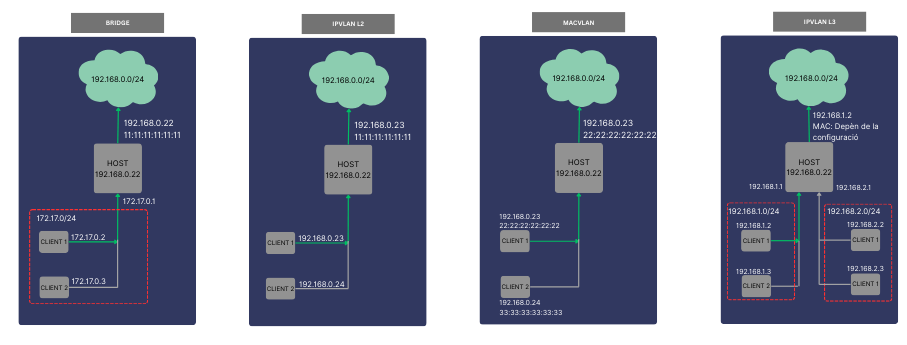
\includegraphics[width=1\textwidth]{img/DockerNetworks.png}
    \caption{La figura mostra el comportament dels diferents drivers de xarxa de Docker (excloent el mode host on directament actua en nom de l'hipervisor).}
    \label{fig:DockerNetworks}
  \end{figure}